%!TEX TS-program = xelatex
% !TeX program = xelatex
%!TEX encoding = UTF-8 Unicode
%----------------------------------------------------------------------------------------
%   Доорх хэсгийг өөрчлөх шаардлагагүй
%----------------------------------------------------------------------------------------
\documentclass[12pt,A4]{report}

\usepackage{fontspec,xltxtra,xunicode}
\setmainfont[Ligatures=TeX]{Times New Roman}
\setsansfont{Arial}

% \usepackage[utf8x]{inputenc}
% \usepackage[mongolian]{babel}
%\usepackage{natbib}
\usepackage{geometry}
%\usepackage{fancyheadings} fancyheadings is obsolete: replaced by fancyhdr. JL
\usepackage{fancyhdr}
\usepackage{float}
\usepackage{afterpage}
\usepackage{graphicx}
\usepackage{amsmath,amssymb,amsbsy}
\usepackage{dcolumn,array}
\usepackage{tocloft}
\usepackage{dics}
\usepackage{nomencl}
\usepackage{upgreek}
\newcommand{\argmin}{\arg\!\min}
\usepackage{mathtools}
\usepackage[hidelinks]{hyperref}

\usepackage{algorithm}
\usepackage{algpseudocode}

\usepackage{listings}
\DeclarePairedDelimiter\abs{\lvert}{\rvert}%
\makeatletter
\usepackage{caption}
\captionsetup[table]{belowskip=0.5pt}
\usepackage{subfiles}

\usepackage{listings}

\usepackage{color}
\definecolor{lightgray}{rgb}{.9,.9,.9}
\definecolor{darkgray}{rgb}{.4,.4,.4}
\definecolor{purple}{rgb}{0.65, 0.12, 0.82}

\lstdefinelanguage{JavaScript}{
  keywords={typeof, new, true, false, catch, function, return, null, catch, switch, var, if, in, while, do, else, case, break},
  keywordstyle=\color{blue}\bfseries,
  ndkeywords={class, export, boolean, throw, implements, import, this},
  ndkeywordstyle=\color{darkgray}\bfseries,
  identifierstyle=\color{black},
  sensitive=false,
  comment=[l]{//},
  morecomment=[s]{/*}{*/},
  commentstyle=\color{purple}\ttfamily,
  stringstyle=\color{red}\ttfamily,
  morestring=[b]',
  morestring=[b]"
}

\lstset{
   language=JavaScript,
   backgroundcolor=\color{lightgray},
   extendedchars=true,
   basicstyle=\footnotesize\ttfamily,
   showstringspaces=false,
   showspaces=false,
   numbers=left,
   numberstyle=\footnotesize,
   numbersep=9pt,
   tabsize=2,
   breaklines=true,
   showtabs=false,
   captionpos=b
}
\renewcommand{\lstlistingname}{Код}
\renewcommand{\lstlistlistingname}{\lstlistingname ын жагсаалт}

\usepackage{color}
\definecolor{codegreen}{rgb}{0,0.6,0}
\definecolor{codegray}{rgb}{0.5,0.5,0.5}
\definecolor{codepurple}{rgb}{0.58,0,0.82}
\definecolor{backcolour}{rgb}{0.99,0.99,0.99}
 
\lstdefinestyle{mystyle}{
    basicstyle=\ttfamily\small,
    backgroundcolor=\color{backcolour},   
    commentstyle=\color{codegreen},
    keywordstyle=\color{magenta},
    numberstyle=\tiny\color{codegray},
    stringstyle=\color{codepurple},
    %basicstyle=\footnotesize,
    breakatwhitespace=false,         
    breaklines=true,                 
    captionpos=b,                    
    keepspaces=false,                 
    numbers=left,                    
    numbersep=10pt,                  
    showspaces=false,                
    showstringspaces=true,
    showtabs=false,                  
    tabsize=2
}
 
\lstset{style=mystyle, label=DescriptiveLabel} 

\let\oldabs\abs
\def\abs{\@ifstar{\oldabs}{\oldabs*}}
\makenomenclature
\begin{document}


%----------------------------------------------------------------------------------------
%   Өөрийн мэдээллээ оруулах хэсэг
%----------------------------------------------------------------------------------------

% Дипломийн ажлын сэдэв
\title{Криптографын зарим алгоритм, программ}
% Дипломын ажлын англи нэр
\titleEng{Some algorithms and programs for cryptography}
% Өөрийн овог нэрийг бүтнээр нь бичнэ
\author{Даянгийн Балжинням}
% Өөрийн овгийн эхний үсэг нэрээ бичнэ
\authorShort{Д. Балжинням}
% Удирдагчийн зэрэг цол овгийн эхний үсэг нэр
\supervisor{Д. Гармаа}
% Хамтарсан удирдагчийн зэрэг цол овгийн эхний үсэг нэр
\cosupervisor{Н. Оюун-Эрдэнэ}

% СиСи дугаар 
\sisiId{20B1NUM0563}
% Их сургуулийн нэр
\university{МОНГОЛ УЛСЫН ИХ СУРГУУЛЬ}
% Бүрэлдэхүүн сургуулийн нэр
\faculty{ХЭРЭГЛЭЭНИЙ ШИНЖЛЭХ УХААН, ИНЖЕНЕРЧЛЭЛИЙН СУРГУУЛЬ}
% Тэнхимийн нэр
\department{МЭДЭЭЛЭЛ, КОМПЬЮТЕРИЙН УХААНЫ ТЭНХИМ}
% Зэргийн нэр
\degreeName{Баклаврын судалгааны ажил}
% Суралцаж буй хөтөлбөрийн нэр
\programeName{Програм хангамж(D061302)}
% Хэвлэгдсэн газар
\cityName{Улаанбаатар}
% Хэвлэгдсэн огноо
\gradyear{2023 оны 11 сар}


%----------------------------------------------------------------------------------------
%   Доорх хэсгийг өөрчлөх шаардлагагүй
%----------------------------------------------------------------------------------------
%----------------------Нүүр хуудастай хамаатай зүйлс----------------------------
\pagenumbering{roman}
\makefrontpage
\maketitle

\doublespace

% Decleration
\begin{huge}
	\textbf{Зохиогчийн баталгаа}
\end{huge} \\ \ \\
\doublespace
Миний бие \@author \ "\@title" \ сэдэвтэй судалгааны ажлыг гүйцэтгэсэн болохыг зарлаж дараах зүйлсийг баталж байна:
\begin{itemize}
	\item Ажил нь бүхэлдээ эсвэл ихэнхдээ Монгол Улсын Их Сургуулийн зэрэг горилохоор дэвшүүлсэн болно.
	\item Энэ ажлын аль нэг хэсгийг эсвэл бүхлээр нь ямар нэг их, дээд сургуулийн зэрэг горилохоор оруулж байгаагүй.
	\item Бусдын хийсэн ажлаас хуулбарлаагүй, ашигласан бол ишлэл, зүүлт хийсэн.
	\item Ажлыг би өөрөө (хамтарч) хийсэн ба миний хийсэн ажил, үзүүлсэн дэмжлэгийг дипломын ажилд тодорхой тусгасан.
	\item Ажилд тусалсан бүх эх сурвалжид талархаж байна.
\end{itemize}
\

Гарын үсэг: \underline{\hspace{5cm}}

Огноо: 	\ \ \underline{\hspace{3cm}}

% Гарчгийг автоматаар оруулна
\setcounter{tocdepth}{1}
\tableofcontents

% Зургийн жагсаалтыг автоматаар оруулна
\listoffigures

% Хүснэгтийн жагсаалтыг автоматаар оруулна
\listoftables

% Кодын жагсаалтыг автоматаар оруулна
\lstlistoflistings

% This puts the word "Page" right justified above everything else.
\newpage
%% \addtocontents{lof}{Зураг~\hfill Хуудас \par}
\newpage
%% \addtocontents{lot}{Хүснэгт~\hfill Хуудас \par}

\renewcommand{\cftlabel}{Зураг}


\doublespace
\pagenumbering{arabic}


% Удиртгалыг оруулж ирэх ба abstract.tex файлд удиртгалаа бичнэ
\begin{abstract}
	\setcounter{secnumdepth}{0}
	Энэхүү дипломын ажилд криптографын янз бүрийн алгоритм, программуудыг системтэйгээр судалсан бөгөөд үндсэн зорилго нь тэдгээрийн үндсэн бүтэц, үйл ажиллагааны механизм, практик хэрэглээг ойлгох явдал байв. Энэхүү судалгааны ажилд уламжлалт болон шинээр гарч ирж буй криптографын алгоритмуудыг судалж, гүйцэтгэл, аюулгүй байдал, үр ашигтай байдалд үндэслэн харьцуулсан судалгааг хийв.\\

	Энэхүү судалгаанд өгөгдлийн шифрлэлтийн стандарт (DES), дэвшилтэт шифрлэлтийн стандарт (AES), Ривест-Шамир-Адлеман (РСА (RSA)), эллиптик муруй криптографи (ECC) зэрэг тэгш хэмтэй болон тэгш хэмт бус криптографын алгоритмуудыг нарийвчлан судалсан.\\

	Төгсөлтийн ажлын практик хэсэгт хэд хэдэн криптографын программуудыг боловсруулж харьцуулсан ба орчин үеийн стандартыг хангасан тоон гарын үсгийн системийг үүлэн технологит суурилан бүтээсэн.
	\section{Зорилго}
	Энэхүү ажилд үүлэн технологит суурилсан тоон гарын үсгийн системийг бүтээж хэрэглэгчэд өөрсдийн цахим гарын үсгээр баталгаажсан файлуудыг интернэтэд хуваалцах боломжийг бүрдүүлэх гол зорилго зорилго тавьсан болно.
	\section{Зорилт}
	\begin{enumerate}
		\item Криптографын сонгодог алгоритмуудыг судлах, эзэмших
		\item Криптографын сонгодог алгоритмууд болон үүлэн технологид суурилсан тоон гарын үсгийн систем бүтээх
		\item Бүрэн бүтэн, хөндөгдөөгүй, эх сурвалжтай файлыг хуваалцах боломжийг бүрдүүлэх
	\end{enumerate}
	\section{Үндэслэл}
	Цахим харилцаа холбоо хурдацтай хөгжиж буй өнөөгийн нийгэмд, хуулийн дагуу хүчин төгөлдөр бичиг баримтыг интернэт сүлжээг ашиглан хуваалцах хэрэг байна. Гэсэн хэдий ч Монголд үүлэн дээр суурилсан тоон гарын үсгийн систем байхгүйгээс хэрэглэгчэд нийцгүй байгаа нь харагдаж байна.

	Дэлхийн банкны мэдээллээр Монгол Улсын иргэдийн дийлэнх хувь нь (2021 оны байдлаар 81.61\%) интернэт хэрэглэгч байгаа нь ийм системийн боломжит цар хүрээг харуулж байна. \footnote{Дэлхийн банкны судалгаа: \url{https://data.worldbank.org/indicator/IT.NET.USER.ZS?end=2021&locations=MN}}
	
	Түүнчлэн, одоо байгаа Клиент программууд нь Windows үйлдлийн системд зориулагдсан байдаг. Энэхүү Windows төвтэй арга нь нийцтэй байдлын асуудалд хүргэдэг. StatCounter Global Stats-аас гаргасан мэдээллээс харахад 2023 оны байдлаар дэлхий даяар үйлдлийн системийн зах зээлийн 30 орчим хувийг macOS болон Linux зэрэг Windows бус платформууд эзэлж байна.\footnote{Үйлдлийн системийн судалгаа: \url{https://gs.statcounter.com/os-market-share/desktop/worldwide}}
	
	Эдгээрийг авч үзвэл хэрэглэгчдийн олон талт хэрэгцээнд нийцсэн үүлэн технологит суурилсан тоон гарын үсгийн системийг хөгжүүлэх шаардлагатай байгаа нь харагдаж байна.

	%	\setcounter{secnumdepth}{0} reverse this command
	\setcounter{secnumdepth}{2}

\end{abstract}



%----------------------------------------------------------------------------------------
%   Дипломын үндсэн хэсэг эндээс эхэлнэ
%----------------------------------------------------------------------------------------
%\addcontentsline{toc}{part}{БҮЛГҮҮД}
% Шинэ бүлэг
\chapter{Онолын судалгаа}
\section{Тэгш хэмт крифтограф}
Тэгш хэмт крифтографт шифрлэлт болон шифр тайлах түлхүүрүүд адил байна. Тэгш хэмт алгоритм нь Тэгш бус хэмт шифрлэлтээс харьцангуй хурдан ажилдаг. Гэвч нууцалсан мэдээллийг тайлж унших түлхүүр болон нууцлах түлхүүр адилхан байх нь харилцагч талууд урьдчилан түлхүүрээ хоорондоо тохиролцох шаардлагыг гаргаж ирдэг. Энэ нь сул тал болох эрсдэлтэй. Хэрвээ гуравдагч этгээд түлхүүрийг олж авбал бүх нууцалсан мэдээллийг үзэх боломжтой болох юм.

Хамгийн түгээмэл хэрэглэгддэг тэгш хэмт шифрлэлтийн алгоритм бол Бельгийн криптографич Жоан Даемен, Винсент Рижмен нарын боловсруулсан Advanced Encryption Standard (AES) юм. AES нь хуучин Data Encryption Standard (DES)-ийг сольсон бөгөөд одоо дэлхий даяар ашиглагдаж байна.\cite{AES}
\subsection{Блокон шифрлэлт}

Хэрвээ эх ба шифрлэгдсэн тексүүдийн огторгуй нь ямар нэг $\sum_{}^{n}$ олонлог байвал тухайн криптографыг блокон шифрлэлт гэнэ. Блокон шифрлэлтэд өгсөн мэдээг тэнцүү \textit{n} урттай хэсгүүдэд хуваан шифрлэдэг.\cite{intro_crypo}

Блок шифрт энгийн текстийн блокийг бүхэлд нь авч, шифрлэгдсэн текстийн блокийг үүсгэхэд ашигладаг. Блокийн хэмжээг ерөнхийдөө шифрийн алгоритмаар тодорхойлно. Ихэнх блок шифрүүдийн хувьд энэ нь ихэвчлэн 64 эсвэл 128 бит байдаг ба зарим тохиолдолд нууцлалыг нэмэх зорилгоор 256, 512 бит ч байж болдог.


Хоёр төрлийн алгоритм ашиглах ба нэг нь шифр хийхэд нөгөө нь тайлахад ашиглагддаг. Эдгээр нь \textit{n} урттай бит болон \textit{k} бит урттай түлхүүрийг авч \textit{n} бит урттай блок үүсгэнэ.\\$E: \{0,1\}^k \times \{0,1\}^n \rightarrow \{0,1\}^n$.
	Тайлах алгоритм \textit{D}-г нууцлах функцийн урвуу гэж тодорхойлж болно.\\ $D: \{0,1\}^k \times \{0,1\}^n \rightarrow \{0,1\}^n$\\
$\forall k \in \{0,1\}^k, \forall m \in \{0,1\}^n, D(k, E(k, m)) = m$\\
	\cite{modern_crypto}

	\subsection{Урсгалын шифрлэлт}
	Урсгалын шифрлэлт гэдэг нь өгөгдлийг урсгал маягаар нэг дор нэг битийг Криптографын алгоритм болон түлхүүрээ ашиглан шифрлэх арга юм. Урсгалын шифрийн давуу тал нь блок шифрлэлтээс харьцангуй хурдан ажиллахаас гадна, хэрэгжүүлэлтэд бага код ордог билээ. Гэсэн хэдий ч орчин үед түгээмэл ашиглагдахаа больсон ба элдэв халдагад түгээмэл өртдөг нь үүнтэй холбоотой. Жишээ нь RC4 гэх Урсгалын шифрлэлтийн алгоритм нь WEB болон WPA хамгаалалтад ашиглагддаг байсан хэдий ч хангалттай сайн хамгаалалт болж чадахгүй байгаа тул, хэрэглээнээс халагдаж байна.

	\section{Өгөгдөл шифрлэлтийн стандарт}
	\subsection{DES алгоритм}
	DES (Data Encryption Standard) нь 1970-аад онд хөгжүүлэгдсэн тэгш хэмт блок шифрлэлтийн алгоритм юм. DES нь 64 бит урттай блок дээр ажиллах ба үүнийг 32-бит урттай хоёр хэсэг $L_{0}, R_{0}$ болгон хувааж, баруун талын 32-бит урттай хэсгийг олон янзын аргаар хувиргаж эцэст нь $L_{0}$-тэй XOR үйлдэл хийнэ. Арван зургаан үе хувиргалтын дараагаар $L_{0}, R_{0}$ нийлүүлж 64 бит шифрлэгдсэн блокийг үүсгэнэ.
	\subsubsection{Шинжүүд}
	\begin{enumerate}
		\item Түлхүүрийн урт: DES нь 56 битийн түлхүүрийг ашигладаг бөгөөд анхандаа хангалттай аюулгүй байдлыг хангадаг гэж бодож байсан ч одоо Brute Force халдлагад маш эмзэгт тооцогддог.
		\item Symmetric Encryption: DES нь шифрлэлт болон шифрийг тайлахад ижил түлхүүр ашигладаг. Тиймээс түлхүүрийг илгээгч, хүлээн авагч хоёулаа мэдэж, нууцлах ёстой.

		\item Блок шифр: DES нь тусдаа бит биш харин өгөгдлийн блокууд дээр ажилладаг. Энэ нь их хэмжээний өгөгдлийг шифрлэх шаардлагатай программуудад тохиромжтой.

		\item DES үйлдлүүд: DES нь  Electronic Codebook (ECB), Cipher Block Chaining (CBC), Cipher Feedback (CFB), Output Feedback (OFB), and Counter (CTR) зэрэг хэд хэдэн үйлдлийн горимыг дэмждэг.

		\item DES нь детерминистик: ижил текст болон ижил түлхүүрийн хувьд шифрлэгдсэн текст үргэлж ижил байх болно.
	\end{enumerate}
	хэдийгээр 3-DES гэж байдаг хэдий ч энэ нь тооцоолол ихээр шаарддаг тул цаашид ашиглагдах нь зогссон.

	\subsection{AES}
	АНУ-ын Стандарт, Технологийн үндэсний хүрээлэн (VIST) 1997 онд өгөгдөл нууцлалын стандарт (DES)-ыг сайжруулах ажлыг эхлүүлж 2001 онд В.Рижмень, Д.Дэймен нарын блокон шифрлэлтийн схемийг дэвшилтэт нууцлалын стандартаар зарласан.\cite{intro_crypo}

	AES нь орлуулах сэлгэлт (substitution-permutation) гэж нэрлэгддэг зарчим дээр суурилдаг бөгөөд программ хангамж болон техник хангамжийн аль алин дээр нь хурдан ажилдаг. Орчин үед шифрлэлтийг хурдан хийх зорилгоор техник хангамж дээр зөвхөн энэ алгоритмд зориулсан хэсэг хүртэл байдаг билээ.
	\subsubsection{Үндсэн үйлдэл}
	\begin{enumerate}
		\item \textbf{SubBytes:}
		      \begin{itemize}
			      \item Байт болгоны байрлалыг солино
			      \item Тухайн мөр баганын мэдээлэл солигдоно
		      \end{itemize}
		      \begin{figure}[h]
			      \centering
			      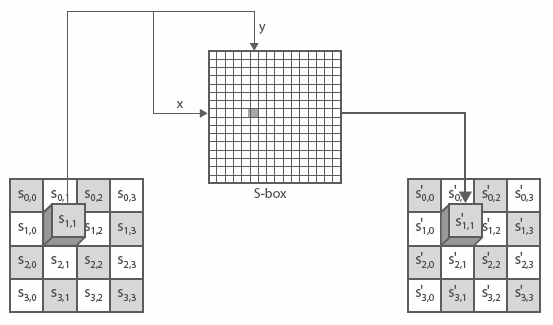
\includegraphics[scale=0.65]{assets/subbytes.png}
			      \caption{SubBytes үйлдэл}
			      \label{fig:subbytes}
		      \end{figure}
		\item \textbf{ShiftRows:}
		      \begin{itemize}
			      \item 1-р мөрийг шилжүүлэхгүй
			      \item 2–р мөрийн байтуудыг зүүн тийш 1 байт шилжүүлнэ
			      \item 3–р мөрийн байтуудыг зүүн тийш 2 байт шилжүүлнэ
			      \item 4–р мөрийн байтуудыг зүүн тийш 3 байт шилжүүлнэ
			      \item Тайлах үйлдлийг хийхдээ баруун тийш шилжүүлэх үйлдлийг хийнэ
		      \end{itemize}
		      \begin{figure}[h]
			      \centering
			      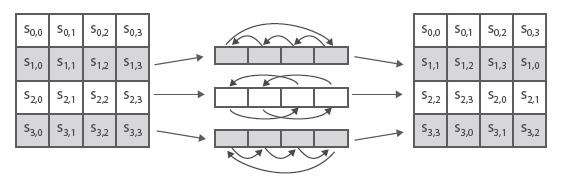
\includegraphics[scale=0.6]{assets/shiftrows.png}
			      \caption{ShiftRows үйлдэл}
			      \label{fig:shiftrows}
		      \end{figure}
		\item \textbf{MixColumns:}
		      \begin{itemize}
			      \item Багана бүр тус тусдаа холигдоно
			      \item Багана болгоны харгалзаа байтууд хоорондоо солигдоно
		      \end{itemize}
		      \begin{figure}[h]
			      \centering
			      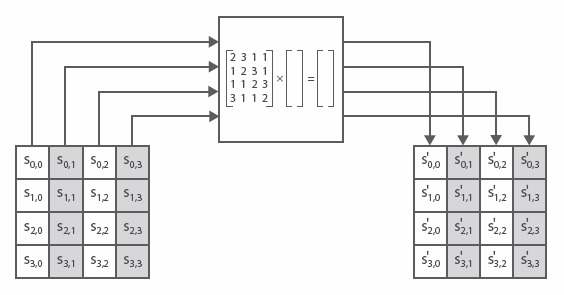
\includegraphics[scale=0.6]{assets/mixcolumns.png}
			      \caption{MixColumns үйлдэл}
			      \label{fig:mixcolumns}
		      \end{figure}
		\item \textbf{AddRoundKey:}
		      \begin{itemize}
			      \item 128 бит XOR үйлдлийг циклийн түлхүүрт ашиглана
			      \item Тайлах үйлдэл хийх бол эсрэгээр гүйцэтгэнэ
		      \end{itemize}
		      \begin{figure}[h]
			      \centering
			      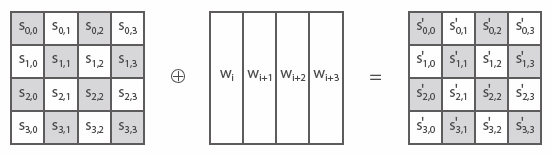
\includegraphics[scale=0.6]{assets/addroundkey.png}
			      \caption{AddRoundKey үйлдэл}
			      \label{fig:addroundkey}
		      \end{figure}
	\end{enumerate}

	\subsubsection{AES-ын нууцлалт}
	\begin{enumerate}
		\item шифрлэх блок ба түлхүүрийн урт, мөчлөгийн тоог сонгох. Шифрлэх блок ба түлхүүрийн урт нь 128, 192, 256 байт байж болох бөгөөд мөчлөгийн тоо нь харгалзан 10, 12, 14 байна.
		\item Шифрлэх текст, түлхүүрийн матриц \textit{T, W, K}-г үүсгэнэ.
		\item Эцсийн мөчлөгөөс бусад мөчлөгийн \textit{T, W, K} матрицуудад \textbf{AES}-н үндсэн үйлдлүүдийг дэс дараалан хийнэ. Харин эцсийн мөчлөгт Mix Columns үйлдлийг хийхгүй.
	\end{enumerate}
	% \subsubsection{Нууцын тайлалт}
	% 4x4 for matrix below
	\begin{center}
		$\begin{bmatrix}
				b_{0} & b_{4} & b_{8}  & b_{12} \\
				b_{1} & b_{5} & b_{9}  & b_{13} \\
				b_{2} & b_{6} & b_{10} & b_{14} \\
				b_{3} & b_{7} & b_{11} & b_{15} \\
			\end{bmatrix}$
	\end{center}
	\subsection{РСА (RSA)}
	РСА (RSA) нь анхны тооны өвөрмөц шинж чанарыг ашигладаг тэгш бус хэмтэй шифрлэлтийн арга юм. Анх 1977 онд танилцуулагдсан ба, өнөөг хүртэл хэрэглээнд хэвээр байгаа. Өнөөдрийн дэлхий даяар мөрдөгдөж байгаа стандарт нь хоёр анхны тооны үржвэр болох модулус нь 2048 бит хэмжээтэй байх ёстой. Энэ нь 617 оронтой тоо байна гэсэн үг юм.
	\begin{itemize}
		\item Хоёр анхны тоо болох $p$ болон $q$ сонгоно.
		\item $n = p*q$ утгыг олно.
		\item $\phi(n) = (p-1)*(q-1)$ утгыг олно.
		\item Дараах нөхцөлийг хангах $e$ тоог сонгоно $1 < e < \phi(n)$ ба хиех$(e, \phi(n)) = 1$.
		\item $d$ нь $d \equiv e^{-1} \mod \phi(n)$ гэж тодорхойлогдоно.
	\end{itemize}

	Нийтийн түлхүүр нь $(e, n)$ болох ба хувийн түлхүүр нь $(d, n)$ болно.\cite{РСА (RSA)}
	
\subsubsection{Нууцлал}
РСА (RSA) алгоритмын нууцлал маш том хэмжээний анхны тоог хоёр тооны үржигдэхүүн болгон задлах дээр тогтдог ба өнөөгийн бидний машины тооцон бодох чадал хараахан хангалттай биш байгаа юм.

\begin{table}[h!]
	\centering
	\caption{Муйхар хүчний алгоритм ашиглан РСА (RSA) нууцлалыг эвдэх нь \cite{Brute-force-РСА (RSA)}}
	\begin{tabular}{|c|c|c|c|}
	\hline
	n & p*q & Оролдого (Хайлт) & Хугацаа (секунд) \\
	\hline
	187 & $11 \times 17$ & 5 & $0.00344800949097$ \\
	913 & $11 \times 83$ & 5 & $0.00358390808105$ \\
	14041 & $19 \times 739$ & 8 & $0.004469871521$ \\
	557009 & $653 \times 853$ & 119 & $0.00167393684387$ \\
	9192907 & $937 \times 9811$ & 159 & $0.00201606750488$ \\
	37675201 & $3907 \times 9643$ & 540 & $0.0139532089233$ \\
	17614895377 & $40559 \times 434303$ & 4252 & $0.117401838303$ \\
	599855115407 & $694789 \times 863363$ & 56166 & $0.712327957153$ \\
	4684589242027 & $837533 \times 5593319$ & 66714 & $1.99000310898$ \\
	6833740248499 & $2565161 \times 2664059$ & 187492 & $2.51408982277$ \\
	91063247464523 & $9577907 \times 35324489$ & 188371 & $8.69724798203$ \\
	\hline
	\end{tabular}
	\end{table}

	Хамгийн сүүлд үржигдэхүүнд задалж чадсан буюу нууцлал нь амжилттай эвдэгдсэн нь РСА (RSA)-250 буюу 829 бит урттай байгаа юм. Фабрис Будот, Пьеррик Гаудри, Ауроре Гилевич, Надия Хенингер, Эммануэль Томе, Пол Циммерманн нараар ахлуулсан судлаачдын баг үүнийг 2020 онд гүйцэтгэсэн. Тооцоололд ойролцоогоор 2700 цөм жил \footnote{Цөм жил гэдэг нь CPU-ний нэг цөмийг бүтэн жил ашигласантай тэнцэнэ.} зарцуулагдсан бөгөөд шигших үе шат нь хуанлийн 35 долоо хоног янз бүрийн машинууд дээр хийгдсэн.

	\begin{figure}[h]
		\centering
		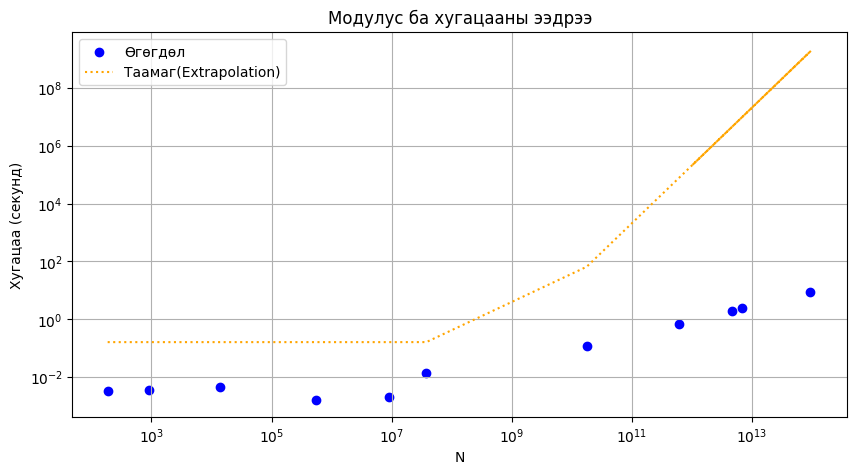
\includegraphics[scale=0.73]{assets/rsacomplexity.png}
		\caption{Хугацааны ээдрээ}
		\label{fig:rsacomplexity}
	\end{figure}

РСА (RSA) үржигдэхүүн задлах нь(factoring) цифрийн тоо нэмэгдэх тусам илтгэгч функцээр хугацааны ээдрээ тооцогдох тул одоогийн байдлаар РСА (RSA) 1024, РСА (RSA) 2048 нь хангалттай аюулгүй байгаа бөгөөд дэлхий нийтээрээ ашиглаж байна. Энэ нь дээрх диаграммаас харагдана.




\chapter{Тайлан боловсруулах зөвлөмж}
\subfile{writing.tex}

\chapter{Бичвэр боловсруулалт}
Бүлгийн гарчгийн дор тухайн бүлэгт юу агуулж байгаа, юуны талаар өгүүлэхийг товч бичих нь баримт бичгийг уншигчдад илүү ойлгомжтой болгодог.
% Бүлгийн дэд гарчиг
\section{Шинэ мөр ба цогцолбор}
Латекс бичих явцад олон хоосон зай, шинэ мөр авахад гаралтын файлд ганцхан хоосон зайгаар дүрсэлж харуулдгаараа бусад засварлагчаас ялгаатай юм.

Шинэ мөр буюу цогцолбор (paragraph) авахдаа хоёр удаа enter товч дарах буюу нэг хоосон мөр үлдээж бичнэ. \par Эсвэл par командыг бичнэ.
\\Харин шинэ мөр авахдаа хоёр ширхэг ургашаа налуу зураас дарааллуулан бичнэ.  Дэлгэрэнгүйг \cite{pharagraph1}-с унш.

Contrary to popular belief, Lorem Ipsum is not simply random text. It has roots in a piece of classical Latin literature from 45 BC, making it over 2000 years old. Richard McClintock, a Latin professor at Hampden-Sydney College in Virginia, looked up one of the more obscure Latin words, consectetur, from a Lorem Ipsum passage, and going through the cites of the word in classical literature, discovered the undoubtable source. Lorem Ipsum comes from sections 1.10.32 and 1.10.33 of "de Finibus Bonorum et Malorum" (The Extremes of Good and Evil) by Cicero, written in 45 BC. This book is a treatise on the theory of ethics, very popular during the Renaissance. The first line of Lorem Ipsum, "Lorem ipsum dolor sit amet..", comes from a line in section 1.10.32.

The standard chunk of Lorem Ipsum used since the 1500s is reproduced below for those interested. Sections 1.10.32 and 1.10.33 from "de Finibus Bonorum et Malorum" by Cicero are also reproduced in their exact original form, accompanied by English versions from the 1914 translation by H. Rackham.

\section{Бичвэр зэрэгцүүлэх}
\subsection{Зүүн тийш зэрэгцүүлэх}
\begin{flushleft}
	Contrary to popular belief, Lorem Ipsum is not simply random text. It has roots in a piece of classical Latin literature from 45 BC, making it over 2000 years old. Richard McClintock, a Latin professor at Hampden-Sydney College in Virginia, looked up one of the more obscure Latin words, consectetur, from a Lorem Ipsum passage, and going through the cites of the word in classical literature, discovered the undoubtable source. Lorem Ipsum comes from sections 1.10.32 and 1.10.33 of "de Finibus Bonorum et Malorum" (The Extremes of Good and Evil) by Cicero, written in 45 BC. This book is a treatise on the theory of ethics, very popular during the Renaissance. The first line of Lorem Ipsum, "Lorem ipsum dolor sit amet..", comes from a line in section 1.10.32.

	The standard chunk of Lorem Ipsum used since the 1500s is reproduced below for those interested. Sections 1.10.32 and 1.10.33 from "de Finibus Bonorum et Malorum" by Cicero are also reproduced in their exact original form, accompanied by English versions from the 1914 translation by H. Rackham.
\end{flushleft}

\subsection{Баруун тийш зэрэгцүүлэх}
\begin{flushright}
	Contrary to popular belief, Lorem Ipsum is not simply random text. It has roots in a piece of classical Latin literature from 45 BC, making it over 2000 years old. Richard McClintock, a Latin professor at Hampden-Sydney College in Virginia, looked up one of the more obscure Latin words, consectetur, from a Lorem Ipsum passage, and going through the cites of the word in classical literature, discovered the undoubtable source. Lorem Ipsum comes from sections 1.10.32 and 1.10.33 of "de Finibus Bonorum et Malorum" (The Extremes of Good and Evil) by Cicero, written in 45 BC. This book is a treatise on the theory of ethics, very popular during the Renaissance. The first line of Lorem Ipsum, "Lorem ipsum dolor sit amet..", comes from a line in section 1.10.32.

	The standard chunk of Lorem Ipsum used since the 1500s is reproduced below for those interested. Sections 1.10.32 and 1.10.33 from "de Finibus Bonorum et Malorum" by Cicero are also reproduced in their exact original form, accompanied by English versions from the 1914 translation by H. Rackham.
\end{flushright}


\section{Хэлбэржилт}
Энэ бүлэгт бичвэрийг хэлбэржүүлэх (format) командуудын талаар дурьдана. Илүү дэлгэрэнгүйг \cite{format1}-с хар.

\subsection{Тодруулах}
\texttt{\textbackslash textbf} командаар бичвэрийг \textbf{тодруулах буюу болд} болгоно.

\subsection{Налуулах}
\texttt{\textbackslash textit} командаар бичвэрийг \textit{бичмэл буюу италик} болгоно.

\subsection{Доогуур зураас}
\texttt{\textbackslash underline} командаар бичвэрийг \textbf{тодруулах буюу болд} болгоно.

\section{URL оруулах}
\texttt{\textbackslash url} команд дотор холбоосыг бичнэ. \url{http://milab.num.edu.mn}


\section{Жагсаалт}
\subsection{Энгийн жагсаалт}
\texttt{\textbackslash begin\{itemize\}} командын дотор энгийн жагсаалтыг бичнэ \cite{list}.
\begin{itemize}
	\item Жагсаалтын эхний элемент
	\item Жагсаалтын хоёрдугаар элемент
	\item Жагсаалтын гуравдугаар элемент
	\item Жагсаалтын дөрөвдүгээр элемент
\end{itemize}

\subsection{Дугаартай жагсаалт}
\texttt{\textbackslash begin\{enumerate\}} командын дотор энгийн жагсаалтыг бичнэ \cite{list}.
\begin{enumerate}
	\item Жагсаалтын эхний элемент
	\item Жагсаалтын хоёрдугаар элемент
	\item Жагсаалтын гуравдугаар элемент
	\item Жагсаалтын дөрөвдүгээр элемент
\end{enumerate}


\chapter{Ишлэл, зүүлт}
\section{Ишлэл}
Ашигласан материал эсвэл номзүйг бичвэр тодор ишлэхдээ cite командаар заалтыг нь оруулна.
Үүний тулд энэ хуудасны хамгийн доор байгаа \textit{Ашигласан материал, ном зүй} хэсэгт
bibitem командыг нэмнэ. \\


Жишээ нь: bibitem\{image1\} Гарчиг, Зохиогчдын нэр, хэвлэсэн он, хэвлэсэн газар

Дээрх жишээнд image1 гэдэг нь ишлэх нэр. Доод талын мөрөнд нь байгаа дарааллын дагуу
ашигласан материалыг бичнэ.

Ишлэхдээ cite командад ишлэх нэрийг дамжуулж өгнө. Жишээ нь cite\{image1\}.
\section{Зүүлт}
Зүүлтийг footnote командаар оруулна \footnote{Энэ холбоосоос зүүлтийн талаар дэлгэрэнгүй унш: \url{https://www.sharelatex.com/learn/Footnotes}}.

\chapter{Зураг}
Зураг оруулахдаа includegraphics командыг ашиглана. Доорх жишээнд figure01.png гэдэг нь зургийн файлын нэр бөгөөд өргөтгөлийг заавал бичих шаардлагагүй. Зургийн файл нь main.tex файлтай нэг фолдерт байх шаардлагатайг анхаарна уу! Дэлгэрэнгүйг \cite{image1}-с үз.


\includegraphics{figure01.png}


\section{Зургийн хэмжээ өөрчлөх}
Хэмжээг томруулахдаа 0-1 хооронд утга ашиглана. Хэрэв 2 гэвэл 2 дахин томроно.
\begin{center}
	includegraphics[scale=0.5]\{figure01\}
\end{center}


\includegraphics[scale=0.9]{figure01}

Өндөр өргөнийг шууд зааж өгч болох бөгөөд дөрвөлжин хаалтан дотор доорх байдлаар бичнэ.
\begin{center}
	includegraphics[width=3cm, height=4cm]\{figure01\}
\end{center}

\includegraphics[width=3cm, height=4cm]{figure01}

\section{Зураг эргүүлэх}
Зургийн эргүүлэхдээ angle параметрт эргүүлэх өнцгийн хэмжээг өгнө.
\begin{center}
	includegraphics[width=3cm, height=4cm, angle=45]\{figure01\}
\end{center}

\includegraphics[width=3cm, height=4cm, angle=45]{figure01}

\section{Зургийн нэр}
Зургын нэрийг begin\{figure\} хооронд includegraphics командтай хамт оруулна Зураг \ref{fig:lion1}-ыг хар.

Энд зургийн нэрээс гадна label-ийг давхар бичиж өгөх шаардлагатай ба энэ нь зургийн дугаараар заалт хийхэд ашиглана. Жишээ нь: Зураг \ref{fig:lion2}

\begin{figure}[h]
	\centering
	
\includegraphics[scale=0.9]{figure01}
	\caption{Зураг голлуулах}
	\label{fig:lion1}
\end{figure}

\section{Зураг голлуулах}
Зургийг голлуулахдаа includegraphics командын өмнө centering
командыг бичээд reflectbox командыг includegraphics болон caption
командуудад үйлчлэхээр оруулна.

\begin{figure}[h]
	
\includegraphics[scale=0.5]{figure01.png}
	\caption{Зургийн нэрийг энд бичнэ}

	\label{fig:lion2}
\end{figure}

\section{Зургийн чанар}
LaTex-т зургийг вектор форматаар (svg, eps) оруулбал хэвлэх болон томруулж харахад зургийн чанар
алдагдахгүй. Тиймээс аль болох вектор зураг оруулж өгвөл зүгээр.

\chapter{Хүснэгт оруулах}
Хүснэгт оруулахад tabular командыг ашигладаг \cite{table}.

\begin{table}[h]
	\centering
	\caption{Хүснэгтийн нэр. Хүснэгтийн нэр хүснэгтийн дээд талд байрлана. }
	\label{my-label}
	\begin{tabular}{|l|l|l|l|l|}
		\hline
		\textbf{Багана1} & \textbf{Багана2}  & \textbf{Багана3} & \textbf{Багана4} & \textbf{Багана5} \\ \hline
		өгөгдөл          & \textit{өгөгдөл1} &                  &                  &                  \\ \hline
		                 &                   &                  &                  &                  \\ \hline
		                 &                   &                  &                  &                  \\ \hline
	\end{tabular}
\end{table}

\section{Хүснэгт зурах хэрэгсэл}
Цэвэр LaTex кодоор Хүснэгт үүсгэхэд харьцангуй төвөгтэй байдаг учир
хялбар хэрэгслийг ашиглаж болно.

Тухайлбал \url{https://www.tablesgenerator.com/} холбоосруу орж хүснэгтийг визуал орчинд зураад үүсгэж өгсөн LaTex кодыг энд хуулж оруулна.

\chapter{Код ба алгоритм оруулах}
Код оруулахдаа begin\{lstlisting\}  ... end\{lstlisting\} командын хооронд бичнэ.

\begin{lstlisting}[language=C, caption=С хэлний кодын жишээ, frame=single]
#include <stdio.h>
#define N 10
/* Block
 * comment */
int main()
{
    int i;
    // Line comment.
    puts("Hello world!");
    for (i = 0; i < N; i++)
    {
        puts("LaTeX is also great for  programmers!");
    }
    return 0;
}
\end{lstlisting}

Мөн кодын эх файлыг шууд оруулж ирж болох бөгөөд доорх командыг бичнэ.

\lstinputlisting[language=C, firstline=11, lastline=16, caption=Кодын файлаас хэсэгчилж оруулах]{src/hello.c}

Мэдээллийн технологи, програм хангамжийн ажлын тайланд алгоримтыг хийсвэр кодын бичиглэлээр оруулах шаардлага гардаг. Дараах жишээгээр (Алгоритм \ref{alg:task_gen}) хийсвэр кодоор хэрхэн бичиж болохыг харуулав. Мөн бичвэр дотроо алгоритмд ашиглаж байгаа $parentId$ хувьсагчийг дурдаж бичиж болдог.

\makeatletter
\newenvironment{megaalgorithm}[1][htb]{%
	\renewcommand{\ALG@name}{Алгоритм}% Update algorithm name
	\begin{algorithm}[#1]%
		}{\end{algorithm}}
\makeatother

\begin{megaalgorithm}
	\caption{Даалгавар үүсгэх алгоритм}\label{alg:task_gen}
	\begin{algorithmic}[1]
		\Function{traverse}{$parentId$}\Comment{parentId--эцэг ойлголтын дугаар}
		\State $children \gets \Call{getChildConceptIds}{parentId$}
			\State $childCount \gets children.count$
		\If{$childCount == 0$}
		\State \textbf{return}
		\EndIf
		\For{$i = 0$ \textbf{to} $childCount$}
		\State \Call{generateTask}{$children_i$}\Comment{Орчуулгын даалгавар үүсгэх}
		\EndFor
		\For{$i = 0$ \textbf{to} $childCount$}
		\State \Call{traverse}{$children_i$}
		\EndFor
		\EndFunction
	\end{algorithmic}
\end{megaalgorithm}

%----------------------------------------------------------------------------------------
%   Дүгнэлт эндээс эхэлнэ
%----------------------------------------------------------------------------------------
\conclusion{Дүгнэлт}
сольсонДүгнэлтийг энд бич


%----------------------------------------------------------------------------------------
%   Дипломын номзүй, хавсралтын хэсэг эндээс эхэлнэ
%----------------------------------------------------------------------------------------

\singlespace
\addcontentsline{toc}{part}{НОМ ЗҮЙ}
\begin{thebibliography}{}
	% Ашигласан материалыг эндээс оруулна
	\bibitem{AES}
	Daemen, J., \& Rijmen, V. (2002). "The Design of Rijndael: AES - The Advanced Encryption Standard." Springer. p.1-2.
	\bibitem{pharagraph1}
	Paragraphs and new lines,  Share LaTex, \url{https://www.sharelatex.com/learn/Paragraphs_and_new_lines}
	\bibitem{intro_crypo}
	Д. Гармаа (2022). "Криптографын үндэс." Улаанбаатар хот.
	\bibitem{modern_crypto}
	Bellare, Mihir; Rogaway, Phillip (11 May 2005), Introduction to Modern Cryptography (Lecture notes), archived (PDF) from the original on 2023-10-30, chapter 3.

\end{thebibliography}


%----------------------------------------------------------------------------------------
%   Хавсралтууд эндээс эхэлнэ
%----------------------------------------------------------------------------------------
\appendix
\addcontentsline{toc}{part}{ХАВСРАЛТ}

% Хавсралтын нэр. Хавсралт гэдэг үг агуулахгүй
\chapter{Шинжилгээ зохиомж}
Хавсралтын агуулга

% Хавсралтын нэр. Хавсралт гэдэг үг агуулахгүй
\chapter{Кодын хэрэгжүүлэлт}

\begin{lstlisting}[language=Python]
	import numpy as np
	 
	def incmatrix(genl1,genl2):
			m = len(genl1)
			n = len(genl2)
			M = None #to become the incidence matrix
			VT = np.zeros((n*m,1), int)  #dummy variable
	 
			#compute the bitwise xor matrix
			M1 = bitxormatrix(genl1)
			M2 = np.triu(bitxormatrix(genl2),1) 
	 
			for i in range(m-1):
					for j in range(i+1, m):
							[r,c] = np.where(M2 == M1[i,j])
							for k in range(len(r)):
									VT[(i)*n + r[k]] = 1;
									VT[(i)*n + c[k]] = 1;
									VT[(j)*n + r[k]] = 1;
									VT[(j)*n + c[k]] = 1;
	 
									if M is None:
											M = np.copy(VT)
									else:
											M = np.concatenate((M, VT), 1)
	 
									VT = np.zeros((n*m,1), int)
	 
			return M
	\end{lstlisting}

\end{document}
